\begin{frame}{Climbing Multistrings: Finding Stationary Points for Ala$_2$}
\begin{tikzpicture}
\pcuad{\textwidth}{\textheight}
    \path(cp) 
    ++(0,0.5) node(g1)[anchor=center]{
        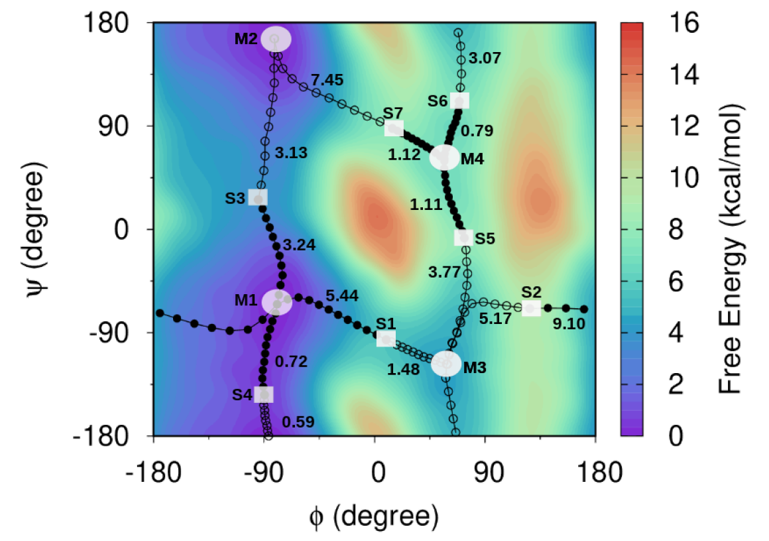
\includegraphics[width=0.85\textwidth]{../ala2network.png}
    };
    \path(g1.north west)
    ++(0,0) node(img1)[anchor=north west]{
        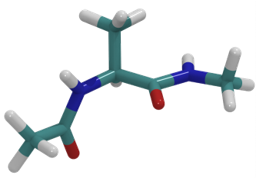
\includegraphics[width=0.25\textwidth]{../ala2m2.png}
    }
    ++(0,0) node(lab1)[anchor=center]{
        {\Large M2}
    };
    \path(g1.south west)
    ++(0,0) node(img2)[anchor=south west]{
        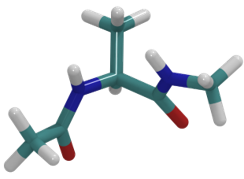
\includegraphics[width=0.25\textwidth]{../ala2m1.png}
    }
    ++(0,0) node(lab1)[anchor=center]{
        {\Large M1}
    };
    \path(g1.south east)
    ++(0,0) node(img3)[anchor=south east]{
        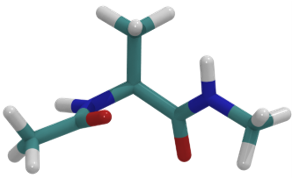
\includegraphics[width=0.25\textwidth]{../ala2m3.png}
    }
    ++(0,0) node(lab1)[anchor=center]{
        {\Large M3}
    };
    \path(g1.north east)
    ++(0,0) node(img3)[anchor=north east]{
        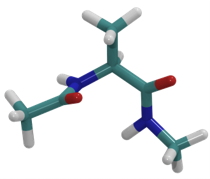
\includegraphics[width=0.25\textwidth]{../ala2m4.png}
    }
    ++(0,0) node(lab1)[anchor=center]{
        {\Large M4}
    };
    \path(se)
    ++(0,0.5) node(att)[anchor=east]{
        {\tiny \textcolor{blue!80!black}{G. Shrivastav and CFA, {\it J Chem Phys} 2019 {\bf 151}:124112}}
    };
\end{tikzpicture}
\end{frame}
